\chapter{The Visual-Inertial Odometry Problem}
\label{ch:intro}

\begin{objectives}
\begin{itemize}
  \item State precisely what visual-inertial odometry estimates and what it cannot estimate.
  \item Understand why an IMU alone drifts, and quantify how fast.
  \item Understand why a monocular camera alone cannot recover metric scale.
  \item Place the MSCKF among the main families of VIO algorithms.
  \item See the complete estimator pipeline that the rest of the notes build piece by piece.
\end{itemize}
\end{objectives}

\section{What odometry is}

\emph{Odometry} is the incremental estimation of a body's motion from its own sensors, without a
prior map and without absolute positioning such as GNSS. The word comes from the wheel odometers of
cars, which count wheel rotations. \emph{Visual-inertial odometry} uses an IMU and one or more
cameras rigidly attached to the body.

At every time $t$ we want the \emph{state}
\begin{equation}
  x(t) = \big(\, p_{wb}(t),\ v_{wb}(t),\ q_{wb}(t),\ b_a(t),\ b_g(t) \,\big),
\end{equation}
namely the position and velocity of the body in a world frame, its orientation, and the slowly
varying biases of the accelerometer and gyroscope. We also want an honest measure of how
uncertain that estimate is. \Cref{ch:rotations} makes the frames and symbols precise. For now, $w$
is a fixed, gravity-aligned world frame and $b$ is the body frame of the IMU.

Odometry differs from \emph{SLAM} (simultaneous localization and mapping) in one important way. A
SLAM system builds a persistent map and recognizes places it has seen before (\emph{loop closure}),
which lets it cancel accumulated drift. An odometry system has no such memory: its error grows
without bound, slowly if it is good and quickly if it is bad. The goal of VIO is to make that growth
as slow as possible, typically well below 1\% of the distance traveled, while running in real time
on modest hardware.

\section{An analogy: the blindfolded walk}

Imagine standing blindfolded in an unfamiliar gymnasium and being asked to walk a 20-meter square
and return to the start. You would rely on your inner ear to sense turning and on the feeling in
your legs to judge distance. Integrating these internal sensations into a running estimate of your
position is \emph{dead reckoning}.

For the first few steps the estimate is good. But your sensors are imperfect: a 90-degree turn
comes out as 87 degrees, and your strides are a little shorter than you think. Each new step is
added on top of a slightly wrong estimate, so the small errors accumulate. After a few minutes you
might believe you are back at the start while actually standing several meters away. This
accumulation is called \emph{drift}.

Now suppose you may lift the blindfold for a tenth of a second every few seconds. The room is dark
except for a few glowing stickers on the walls. You do not know where the stickers are, but by
watching how they shift between glimpses you can infer how you moved, and correct the walking
estimate. That is visual-inertial odometry: the inner ear is the IMU, the glimpses are camera
images, and the stickers are visual features.

Two details of the analogy carry over exactly. First, the glimpses are \emph{relative}: they tell
you how you moved between glimpses, not where you are in some absolute sense, so drift is slowed
but never eliminated. Second, you need both senses. Without the glimpses, drift is fast. Without
the inner ear, a single glimpse cannot tell whether a sticker is small and near or large and far.

\section{The sensors and their weaknesses}

\subsection{The inertial measurement unit}

An IMU contains a three-axis gyroscope and a three-axis accelerometer. Neither measures position.
\begin{itemize}
  \item The \textbf{gyroscope} measures the angular velocity $\omega$ of the body, in rad/s,
        expressed in the body frame.
  \item The \textbf{accelerometer} measures \emph{specific force}: the non-gravitational force per
        unit mass acting on the sensor. At rest on a table it reads $+9.81~\mathrm{m/s^2}$
        \emph{upward}, because the table pushes up on it, and in free fall it reads zero.
        \Cref{ch:imu} explains this carefully.
\end{itemize}
IMUs are fast (typically 100--1000 Hz), cheap, self-contained, insensitive to lighting and
texture, and their measurements are \emph{metric}: an acceleration in $\mathrm{m/s^2}$ carries
an absolute scale. But to get position you must integrate angular rate once to get attitude, then
rotate the specific force into the world frame, add gravity, and integrate twice. Any error in the
sensor or in the attitude is integrated as well.

\subsection{How fast inertial errors grow}

Three error sources dominate short-term inertial drift. The derivations are one-liners, and the
resulting growth laws (\cref{fig:dr-drift}) are worth memorizing.

\begin{enumerate}
  \item \textbf{Accelerometer bias $b_a$.} A constant acceleration error integrated twice gives a
        position error $\tfrac12 b_a t^2$.
  \item \textbf{Initial tilt error $\delta\theta_0$.} If the estimated attitude is tilted by a small
        angle $\delta\theta_0$, the $9.81~\mathrm{m/s^2}$ gravity compensation is applied along a
        slightly wrong axis. A component $g\,\delta\theta_0$ of gravity leaks into the horizontal
        acceleration, and the position error grows as $\tfrac12 g\,\delta\theta_0\, t^2$.
  \item \textbf{Gyroscope bias $b_g$.} Now the tilt itself grows linearly, $\delta\theta(t) = b_g t$,
        so the leaked acceleration is $g b_g t$, and integrating twice gives
        $\tfrac16 g\, b_g t^3$.
\end{enumerate}

\begin{figure}[t]
  \centering
  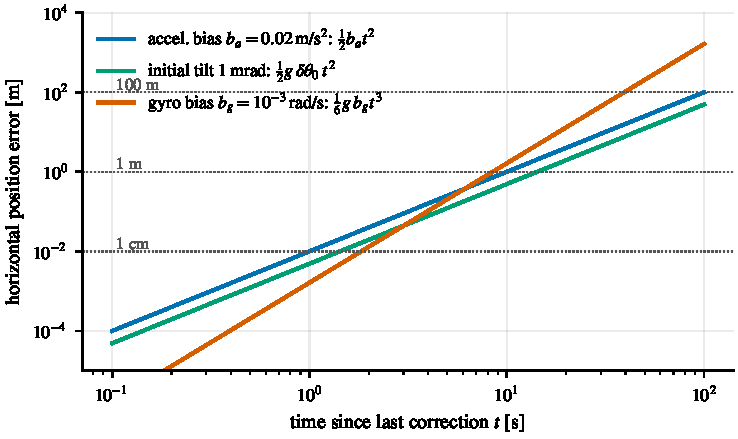
\includegraphics[width=0.86\textwidth]{fig_dr_drift.pdf}
  \caption{Deterministic dead-reckoning drift from three error sources of a consumer-grade IMU.
  A gyro bias of $10^{-3}$~rad/s ($\approx 0.06\,^\circ$/s) produces more than a meter of error
  after ten seconds and hundreds of meters after one minute. The cubic law is why attitude
  accuracy dominates inertial navigation.}
  \label{fig:dr-drift}
\end{figure}

With $b_g = 10^{-3}$~rad/s, a modest value for a MEMS gyroscope, the gyro term alone gives
$1.6$~m after 10~s and $353$~m after 60~s. Random sensor noise adds error that grows in a
similar way. \Cref{ch:errordyn} derives that the position \emph{standard deviation} due to
accelerometer white noise grows as $t^{3/2}$, due to gyroscope white noise as $t^{5/2}$, and due to
the gyroscope bias random walk as $t^{7/2}$.

\begin{keyidea}[inertial navigation is an attitude problem]
Because gravity is large (about $9.81~\mathrm{m/s^2}$) compared with typical accelerometer errors,
a tilt of one milliradian costs as much as an accelerometer bias of about
$10~\mathrm{mm/s^2}$. Position accuracy is therefore limited mostly by attitude accuracy. Any aiding
sensor that constrains roll and pitch, as a camera does, pays off enormously.
\end{keyidea}

\subsection{The camera}

A camera measures the \emph{directions} (bearings) of light rays arriving from the scene. A point
$p_f$ in the world appears in the image at the projection of its camera-frame coordinates
$p_c = (X_c, Y_c, Z_c)$:
\begin{equation}
  z = \begin{bmatrix} X_c/Z_c \\ Y_c/Z_c \end{bmatrix}.
\end{equation}
Because images are measurements of fixed scene geometry, they do not drift the way integrated
inertial data does. But a single camera has a fundamental blind spot.

\begin{proposition}[Monocular scale ambiguity]
\label{prop:scale-ambiguity}
Let a camera with poses $(R_i, p_i)$, $i = 1, \dots, M$, observe points $p_{f,j}$. For any $s > 0$, the
scaled configuration with poses $(R_i, s\,p_i)$ and points $s\,p_{f,j}$ produces exactly the same
images.
\end{proposition}
\begin{proof}
In camera $i$, the scaled point has coordinates
$R_i\T(s\,p_{f,j} - s\,p_i) = s\, R_i\T(p_{f,j} - p_i)$. The projection divides the first two
coordinates by the third, so the factor $s$ cancels.
\end{proof}

A camera alone therefore recovers the trajectory and the scene only up to an unknown global scale.
A photograph of a toy car from 10~cm can be identical to a photograph of a real car from 4~m. Cameras
also fail under motion blur, in darkness, against texture-less surfaces such as white walls, and in
scenes dominated by moving objects.

\subsection{Why the combination works}

\begin{table}[t]
\centering\small
\begin{tabularx}{\textwidth}{@{}>{\raggedright\arraybackslash}X >{\raggedright\arraybackslash}X >{\raggedright\arraybackslash}X@{}}
\toprule
 & \textbf{IMU} & \textbf{Monocular camera} \\
\midrule
Rate & 100--1000 Hz & 10--60 Hz \\
Measures & angular rate, specific force & bearings to scene points \\
Scale & metric & unknown (\cref{prop:scale-ambiguity}) \\
Drift & fast ($t^2$ to $t^3$) & slow, relative to the scene \\
Gravity direction & observable (at rest or on average) & not observable \\
Fails when & always drifts; saturates on impacts & blur, darkness, no texture, pure rotation \\
\bottomrule
\end{tabularx}
\caption{The IMU and the camera fail in complementary ways.}
\label{tab:sensor-complement}
\end{table}

\Cref{tab:sensor-complement} summarizes the complementarity. The camera bounds the inertial drift by
constraining the motion between images. The IMU supplies metric scale, the direction of gravity
(and hence absolute roll and pitch), high-rate motion between frames, and robustness during brief
visual outages. Scale becomes observable because the accelerometer measures acceleration in
$\mathrm{m/s^2}$: scaling a trajectory by $s$ scales its acceleration by $s$, which the
accelerometer would notice. The exception is unaccelerated motion. At constant velocity, the
scale is unobservable again, which is one of several \emph{degenerate motions} studied in
\cref{ch:observability}.

Even fused, four directions remain unobservable: the three components of global position, and the
rotation about the gravity vector (global yaw). Neither sensor senses where the origin is or which
way north is. VIO estimates these relative to the starting pose, and they drift.

\section{Why fusion is hard}

The difficulty of VIO comes from several sources acting at once.
\begin{enumerate}
  \item \textbf{Nonlinearity.} Rotations enter the equations through products and trigonometric
        functions, and the camera projection divides by depth.
  \item \textbf{Curved state spaces.} Orientations do not live in a vector space. You cannot add
        two rotations, and every estimator must deal with this (\cref{ch:lie}).
  \item \textbf{Multi-rate, asynchronous data.} The IMU runs at 200~Hz and the camera at 20~Hz,
        and every measurement must be processed in timestamp order.
  \item \textbf{Unknown scene.} The 3D positions of the visual features are unknown and must be
        estimated, or eliminated, along with the motion.
  \item \textbf{Outliers.} Feature tracks fail, latch onto moving objects, or slide along edges.
  \item \textbf{Unobservability.} Some directions of the state cannot be determined. A careless
        estimator can become falsely confident about them, which is the consistency problem of
        \cref{ch:observability}.
  \item \textbf{Real time.} All of this must run at camera rate, deterministically, on embedded
        processors.
\end{enumerate}

\section{A map of the field}

VIO algorithms differ along three main axes.

\paragraph{Loosely vs.\ tightly coupled.} A loosely coupled system runs a vision-only pipeline
that produces up-to-scale poses and fuses those poses with the IMU. A tightly coupled system feeds
the raw visual measurements (feature positions in the image) directly into a single estimator
together with the inertial data. Tight coupling is more accurate and more robust, because the IMU
helps the vision part and correlations are handled correctly. All modern high-accuracy systems,
and this project, are tightly coupled.

\paragraph{Filtering vs.\ optimization.} \emph{Filtering} approaches (EKF-based) process each
measurement once, keep a Gaussian belief over a bounded state, and discard the past. They are fast
and have predictable cost. \emph{Optimization} approaches solve a nonlinear least-squares problem
over a sliding window of recent states, relinearizing as needed, and summarize discarded states as
a prior (marginalization). They are typically more accurate per frame but more expensive and more
complex. The two families are closer than they appear: the MSCKF is equivalent to a single
Gauss--Newton iteration over a sliding window of poses with the landmarks marginalized
(\cref{ch:msckfupdate}).

\paragraph{Feature-based vs.\ direct.} Feature-based systems extract and track sparse keypoints and
use their image coordinates as measurements. Direct systems use pixel intensities themselves
(photometric error).

\begin{table}[t]
\centering\small
\begin{tabularx}{\textwidth}{@{}l l >{\raggedright\arraybackslash}X@{}}
\toprule
\textbf{System} & \textbf{Family} & \textbf{Notes} \\
\midrule
EKF-SLAM / MonoSLAM~\cite{davison2007monoslam} & filter, landmarks in state & cost grows quadratically with landmarks \\
MSCKF~\cite{mourikis2007msckf, li2013msckf2} & filter, poses in state & landmarks eliminated by nullspace projection; this project \\
MSCKF-VIO~\cite{sun2018msckfvio} & filter (stereo MSCKF) & open-source, fast flight; good engineering reference \\
OpenVINS~\cite{geneva2020openvins} & filter (MSCKF + SLAM features) & research platform with excellent documentation \\
ROVIO~\cite{bloesch2015rovio} & filter, direct & photometric patches in an iterated EKF \\
OKVIS~\cite{leutenegger2015okvis} & optimization, keyframes & sliding-window bundle adjustment \\
VINS-Mono~\cite{qin2018vins} & optimization & preintegration, robust initialization, loop closure \\
ORB-SLAM3~\cite{campos2021orbslam3} & optimization + map & full visual-inertial SLAM with relocalization \\
\bottomrule
\end{tabularx}
\caption{Representative visual-inertial estimators.}
\label{tab:vio-systems}
\end{table}

\section{Why the MSCKF}

In EKF-SLAM every tracked landmark adds three variables to the state. Covariance updates cost
$\mathcal{O}(n^2)$ to $\mathcal{O}(n^3)$ in the state size $n$, so a few hundred landmarks quickly
exhaust a real-time budget, and landmark initialization from a single camera is awkward because
depth is unknown at first sight.

The \textbf{Multi-State Constraint Kalman Filter} of Mourikis and Roumeliotis~\cite{mourikis2007msckf}
keeps instead a sliding window of past IMU poses, called \emph{clones}, taken at image times. When a
feature has been tracked across several clones, its observations constrain those poses relative to
one another. The feature's 3D position is triangulated temporarily, then algebraically
eliminated from the linearized equations by projecting onto the left nullspace of its Jacobian
(\cref{ch:msckfupdate}). The landmark never enters the state. The result:
\begin{itemize}
  \item cost linear in the number of features and bounded by the window size;
  \item no need to initialize landmark depth inside the filter;
  \item all the geometric information of each feature track is used exactly once.
\end{itemize}
These properties make the MSCKF the canonical filter-based VIO and an excellent vehicle for
learning, because it requires every ingredient of the field to be understood and nothing more.

\section{The estimator at a glance}

\begin{figure}[t]
\centering
\begin{tikzpicture}[node distance=7mm and 11mm]
  \node[block] (imu) {IMU\\ \footnotesize 200 Hz};
  \node[block, right=of imu] (prop) {Nominal propagation\\ \footnotesize Ch.~\ref{ch:strapdown}};
  \node[block, right=of prop] (cov) {Covariance propagation\\ \footnotesize Ch.~\ref{ch:errordyn}};
  \node[block, below=10mm of imu] (cam) {Camera\\ \footnotesize 20 Hz};
  \node[block, right=of cam] (front) {Front end: detect,\\ track, reject\\ \footnotesize Ch.~\ref{ch:frontend}};
  \node[block, right=of front] (clone) {Clone pose,\\ augment $P$\\ \footnotesize Ch.~\ref{ch:cloning}};
  \node[block, below=10mm of clone] (upd) {MSCKF update:\\ triangulate, project,\\ gate, update\\ \footnotesize Ch.~\ref{ch:msckfupdate}};
  \node[block, left=of upd] (inj) {Inject, reset,\\ marginalize\\ \footnotesize Ch.~\ref{ch:eskf}, \ref{ch:cloning}};
  \node[block, below=8mm of inj, fill=white] (out) {Pose, velocity,\\ biases, covariance};
  \coordinate (L) at ($(cam.west)+(-7mm,0)$);
  \coordinate (T) at ($(imu.north)+(0,6mm)$);
  \draw[->] (imu) -- (prop);
  \draw[->] (prop) -- (cov);
  \draw[->] (cam) -- (front);
  \draw[->] (front) -- node[note, above]{tracks} (clone);
  \draw[->] (cov) -- (clone);
  \draw[->] (clone) -- (upd);
  \draw[->] (upd) -- (inj);
  \draw[->] (inj) -- (out);
  \draw[->, dashed] (inj.west) -| (L) -- (L |- T) -| node[note, above, pos=0.25]{corrected state feeds back into propagation} (prop.north);
\end{tikzpicture}
\caption{Data flow of the monocular MSCKF built in these notes.}
\label{fig:pipeline}
\end{figure}

\Cref{fig:pipeline} shows the whole estimator. Between images, each IMU sample advances the nominal
state with the nonlinear kinematics and grows the error covariance. When an image arrives, the
filter propagates exactly to the image timestamp, appends a clone of the current pose, and updates
the feature tracks. Tracks that have ended, or whose oldest observation is about to leave the window,
are triangulated and converted into constraints between clones. The update corrects the IMU state and
all clones together, the correction is injected into the nominal state, and the oldest clone is
removed when the window is full. \Cref{ch:planar} builds a complete miniature of this pipeline for a robot moving in a plane,
small enough to derive by hand and to run as a short Python script; it is the place to look whenever the general chapters
feel abstract.

\begin{projectlink}[the road map]
The project builds this pipeline from the bottom up: the Lie group toolkit (M2), the data
stream (M3), inertial propagation (M4--M5), a filter tested against synthetic pose measurements
(M6--M7), the visual front end (M8--M9), and finally the MSCKF (M10a--M10b). Each layer is tested
in isolation before the next is added, so that any later failure can be localized.
\end{projectlink}

\section{The EuRoC benchmark}

The European Robotics Challenge (EuRoC) MAV dataset~\cite{burri2016euroc} is the standard VIO
benchmark. A hexacopter carries a stereo pair of global-shutter cameras ($752 \times 480$, 20~Hz)
and an ADIS16448 MEMS IMU (200~Hz), hardware-synchronized and calibrated. Eleven sequences fly
through an industrial machine hall (MH\_01 to MH\_05) and a motion-capture room (V1\_01 to V2\_03),
graded easy, medium and difficult by speed, lighting and texture. Ground truth comes from a laser
tracker or a motion-capture system. \Cref{app:euroc} documents the file formats and calibration
values the project uses.

\begin{takeaways}
\begin{itemize}
  \item VIO estimates pose, velocity and IMU biases from an IMU and a camera, with no map and no
        absolute positioning, and its error grows without bound.
  \item Inertial drift is dominated by attitude error: a gyro bias produces position error growing
        like $t^3$.
  \item A monocular camera observes the scene only up to scale. The accelerometer supplies the
        scale, provided the body accelerates.
  \item Global position and yaw remain unobservable even with both sensors.
  \item The MSCKF keeps a sliding window of past poses rather than landmarks, which bounds its cost
        while using every feature track.
\end{itemize}
\end{takeaways}

\begin{exercises}
  \item A MEMS accelerometer has a bias of $5~\mathrm{mg}$ ($1\,\mathrm{mg} = 9.81\times10^{-3}~\mathrm{m/s^2}$).
        How long can you dead-reckon before the position error exceeds 1~m? What gyro bias produces
        the same error at the same time?
  \item Prove that the gravity leak produced by a constant tilt error $\delta\theta_0$ is
        $g\,\delta\theta_0$ to first order. What is the exact expression, and at what tilt does the
        first-order formula err by 1\%?
  \item Extend \cref{prop:scale-ambiguity}: show that applying a common rigid transformation
        $(R, t)$ to all camera poses and points also leaves the images unchanged. How many
        unobservable degrees of freedom does a monocular camera have? Which of them does an IMU
        remove, and why?
  \item A drone hovers perfectly still for 30~s. Which states can a VIO system estimate during that
        time, and which cannot be distinguished from each other? (Revisit this after
        \cref{ch:observability}.)
  \item Read the abstract and introduction of~\cite{mourikis2007msckf}. In two sentences, state the
        problem with EKF-SLAM that the paper claims to solve, and the key idea of the solution.
\end{exercises}
